\appendix
\section{Funkce sinus, kosinus, arkussinus, akouskosinus}\label{appa}
\begin{figure}[h]%
    \centering
    {{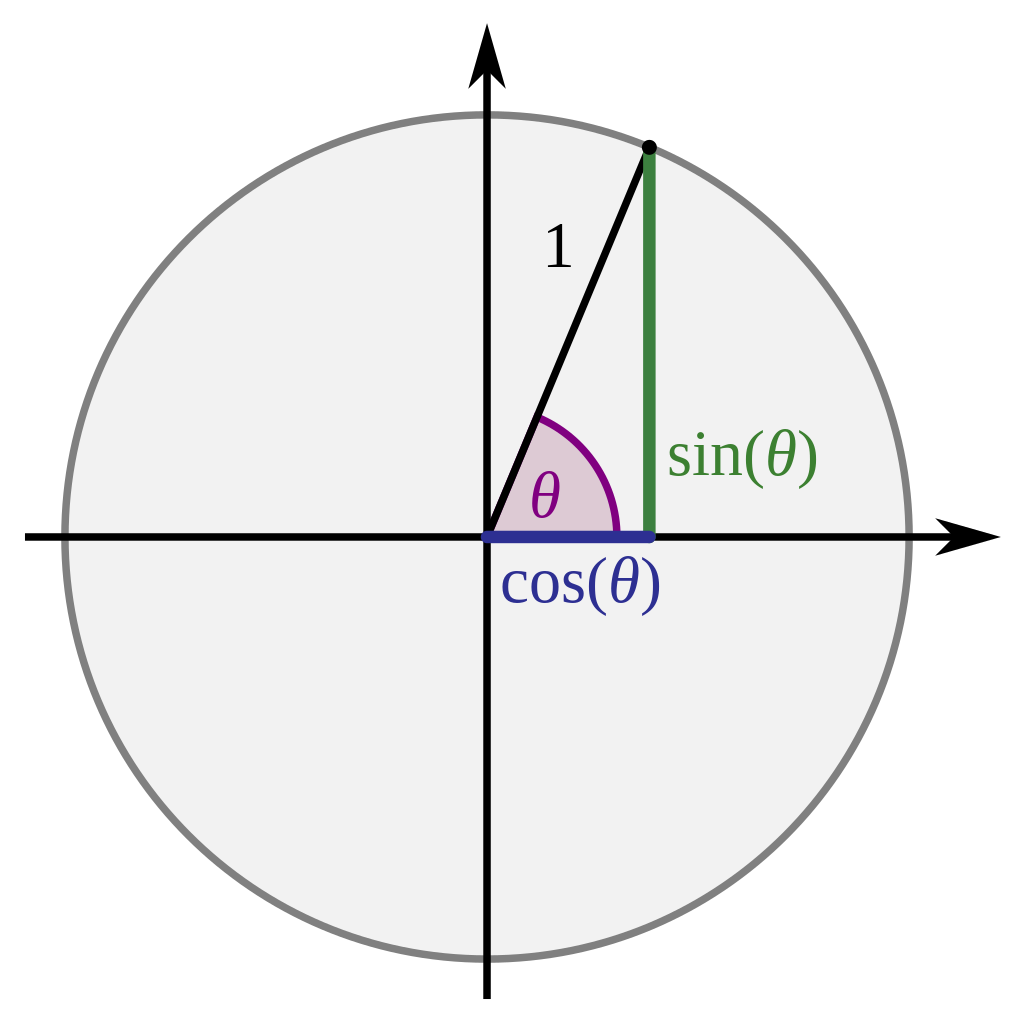
\includegraphics[height=4cm]{images/jednotkova_kruznice.png} }}%
    \qquad
    {{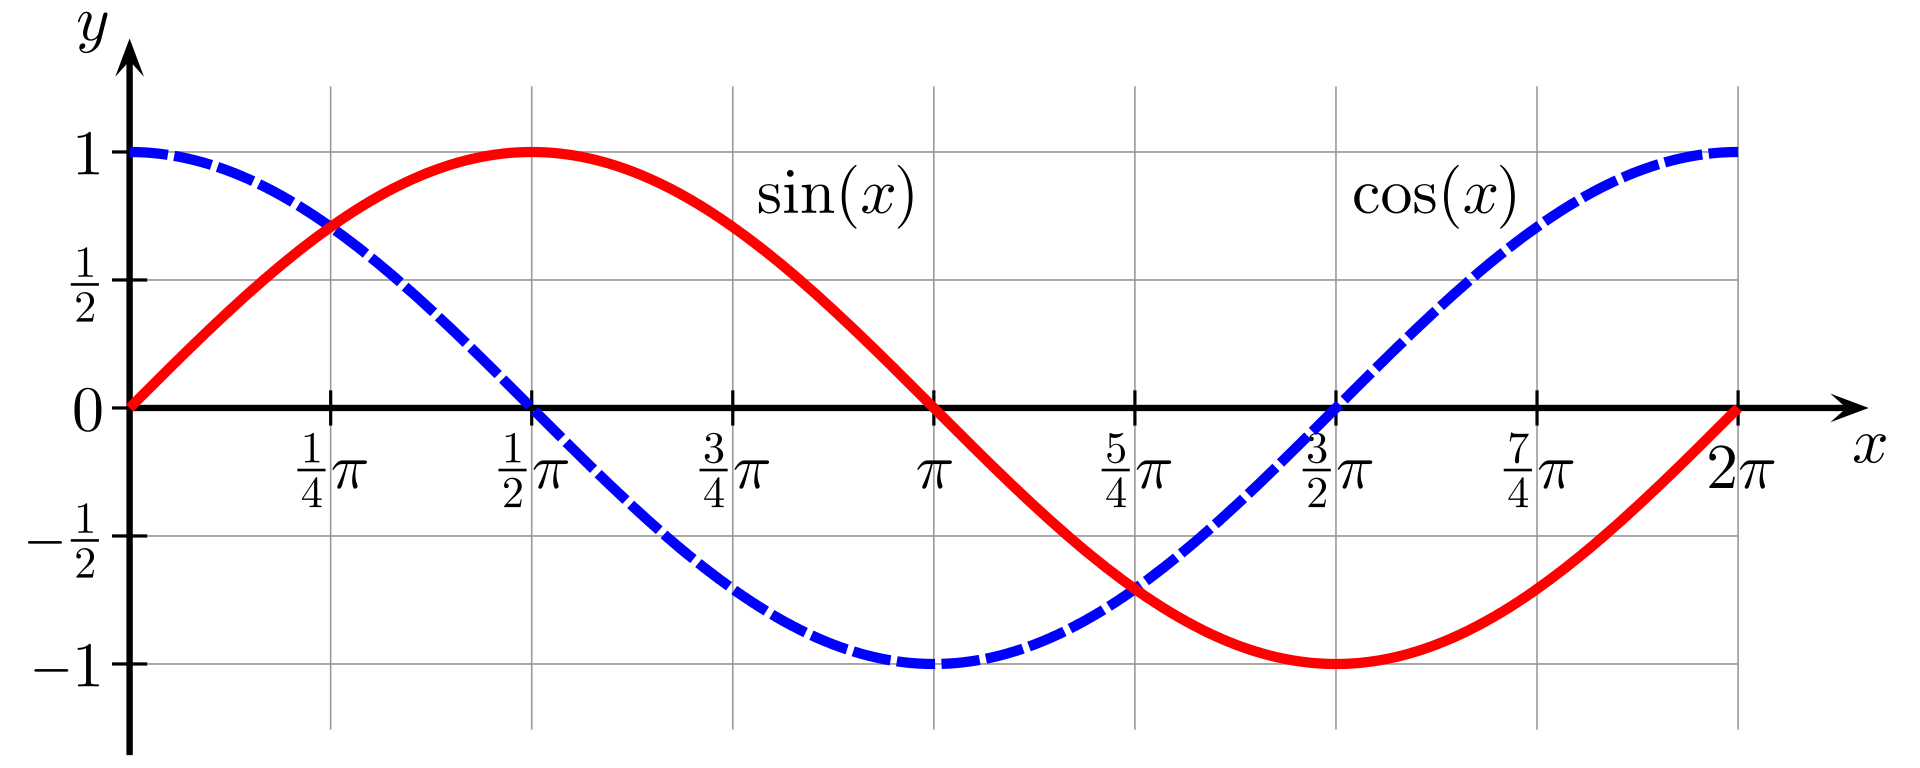
\includegraphics[height=4cm]{images/prubeh.png} }}%
\end{figure}

\begin{figure}[h]%
    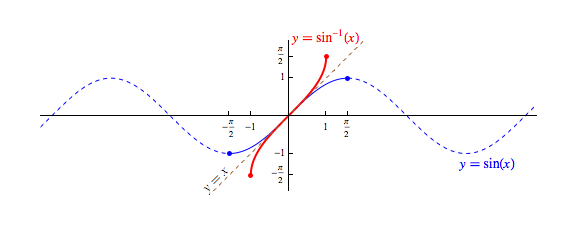
\includegraphics[width=0.5\linewidth]{arcsine.png}
    \hfill
    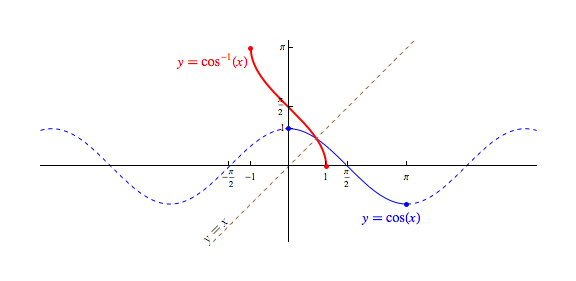
\includegraphics[width=0.5\linewidth]{arccosine.png}
\end{figure}

\begin{pozn}[Základní hodnoty goniometrických funkcí]\,\\
    \begin{tabularx}{\textwidth}{| p{0.087\textwidth} || p{0.081\textwidth} | p{0.081\textwidth} |
    p{0.081\textwidth} | p{0.081\textwidth} | p{0.081\textwidth} | p{0.081\textwidth} | p{0.081\textwidth}
    | p{0.081\textwidth} |}
    \hline
    $\beta$ [$^\circ$] & 0 & 30 & 45 & 60 & 90 & 180 & 270 & 360 \\
    \hline
    $\alpha$ [rad] & 0 & $\frac{\pi}{6}$ & $\frac{\pi}{4}$ & $\frac{\pi}{3}$ & $\frac{\pi}{2}$ & $\pi$ & $\frac{3\pi}{2}$ & $2\pi$\\
    \hline
    $\sin \alpha$ & 0 & $\frac{1}{2}$ & $\frac{\sqrt{2}}{2}$ & $\frac{\sqrt{3}}{2}$ & 1 & 0 & $-1$ & 0\\
    \hline
    $\cos \alpha$ & 1 & $\frac{\sqrt{3}}{2}$ & $\frac{\sqrt{2}}{2}$ & $\frac{1}{2}$ & 0 & $-1$ & 0 & 1\\
    \hline
    $\tg \alpha$ & 0 & $\frac{\sqrt{3}}{3}$ & 1 & $\sqrt{3}$ & -- & 0 & -- & 0\\
    \hline
    $\cotg \alpha$ & -- & $\sqrt{3}$ & 1 & $\frac{\sqrt{3}}{3}$ & 0 & -- & 0 & --\\
    \hline
    \end{tabularx}
\end{pozn}
